\documentclass[conference]{IEEEtran}
\IEEEoverridecommandlockouts
% The preceding line is only needed to identify funding in the first footnote. If that is unneeded, please comment it out.
\usepackage{cite}
\usepackage[utf8]{vietnam}
\usepackage{amsmath,amssymb,amsfonts}
\usepackage{algorithmic}
\usepackage{graphicx}
\usepackage{textcomp}
\usepackage{hyperref}
\usepackage{xcolor}
\usepackage{placeins}
\def\BibTeX{{\rm B\kern-.05em{\sc i\kern-.025em b}\kern-.08em
    T\kern-.1667em\lower.7ex\hbox{E}\kern-.125emX}}
\begin{document}

\title{Báo cáo đồ án Nhập môn Thị giác máy tính (CS231.N11) - Xóa nền bằng phân đoạn màu theo phương pháp Contour Detection}



\author{\IEEEauthorblockN{Lâm Minh Tuấn}
\IEEEauthorblockA{\textit{Trường Đại học Công nghệ Thông tin - ĐHQG TP.HCM} \\
20520843@gm.uit.edu.vn\\
}
}

\maketitle


\section{Giới thiệu bài toán và lý do chọn bài toán}
Xóa nền là một trong những tác vụ phổ biến và quan trọng nhất trong các lĩnh vực Thị giác máy tính và Xử lý ảnh. Ta có thể bắt gặp ứng dụng của việc xóa nền ở bất cứ đâu trên các nền tảng công nghệ như Zoom, TikTok, Instagram, Facebook… Ngoài ra, xóa nền để phát hiện tiền cảnh còn được ứng dụng vào thực tiễn như mã hóa video dựa trên nội dung, giám sát giao thông, nhận dạng chuyển động theo thời gian thực, tương tác người-máy… Bài toán xóa nền chưa bao giờ là một bài toán đơn giản do trên thực tế, các hình ảnh mà ta đưa vào thực hiện xóa nền để có thể áp dụng vào thực tiễn đều là những hình ảnh đời thật với màu sắc phức tạp, đổ bóng, độ tương phản thấp… gây khó khăn cho máy tính. Vì vậy hiện nay phương pháp xóa nền tốt nhất chính là áp dụng Học sâu và Mạng thần kinh tích chập, tuy nhiên do giới hạn phạm vi của môn học, em sẽ không dùng các kĩ thuật liên quan đến Học máy như hai phương pháp trên mà chỉ dùng những phương pháp xử lý trên ảnh đã được học để có thể thực hiện công việc xóa nền với kết quả tương đối. Một trong những phương pháp có thể vận dụng để xóa nền chính là Contour Detection.
\section{Khái niệm đường viền (Contour) và ý tưởng thuật toán}
Đường viền có thể được định nghĩa đơn giản là một đường cong nối tất cả các điểm liên tục, có cùng màu hoặc cường độ màu sắc. Khu vực có cùng màu hoặc cường độ đồng nhất này bao quanh đối tượng mà ta coi là chủ thể. Về cơ bản, thuật toán Contour Detection hoạt động tương tự như các thuật toán phát hiện cạnh nhưng các cạnh phải tạo thành một đường cong khép kín thì thuật toán Contour Detection mới xem đó là đường viền. Để xóa nền bằng thuật toán này, ta chỉ cần xem (các) đối tượng nằm trong đường viền lớn nhất là chủ thể cần giữ lại, và phần hình nằm ngoài đường viền lớn nhất này ta sẽ xem là nền, do đó ta xóa phần hình nằm ngoài này và kết quả ta thu được chủ thể với nền đã được xóa đi.

\section{Thuật toán}

\subsection{Đọc ảnh và chuyển về ảnh xám}
Chuyển về ảnh xám rất quan trọng để chuẩn bị cho các bước tiếp theo. Chuyển bức ảnh ba kênh màu thành một kênh màu để ta có thể phân ngưỡng giúp cho thuật toán phát hiện đường viền hoạt động một cách đúng đắn.
\begin{figure}[!htb]
\centerline{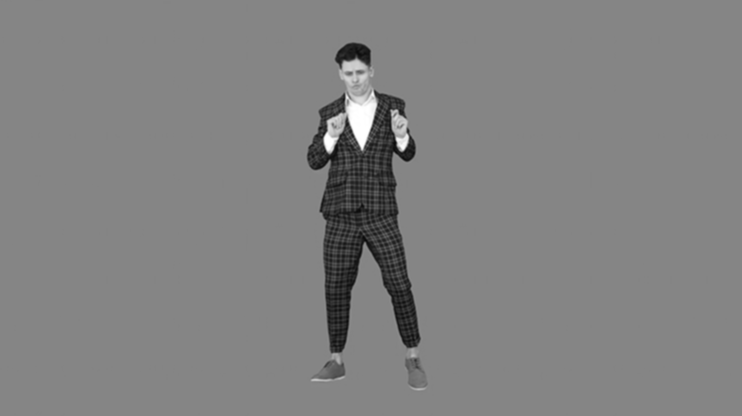
\includegraphics[scale=0.4]{anhxam.png}}
\caption{Ảnh xám.}
\label{fig}
\end{figure}
 \FloatBarrier
\subsection{Nhị phân hóa ảnh}
Nhị phân hóa các giá trị xám trong ảnh thành đen hoặc trắng, điều này làm nổi bật các đối tượng ta quan tâm giúp cho thuật toán tìm đường viền hoạt động hiệu quả hơn.
\begin{figure}[!htb]
\centerline{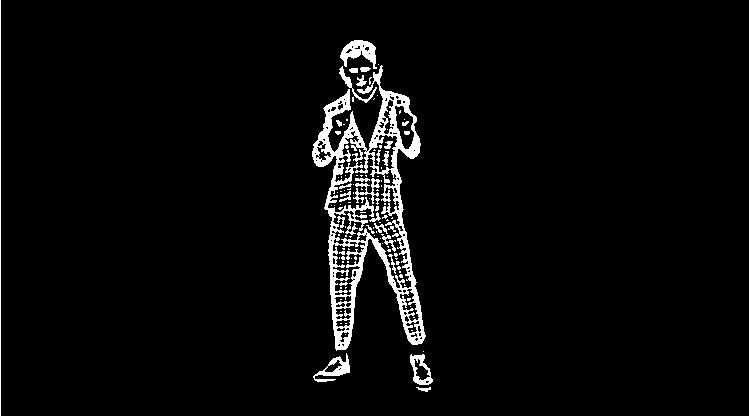
\includegraphics[scale=0.4]{anhnhiphan.png}}
\caption{Ảnh đã được nhị phân hóa.}
\label{fig}
\end{figure}
 \FloatBarrier
\subsection{Áp dụng các thuật toán tìm cạnh}
Áp dụng các thuật toán tìm cạnh như Canny hoặc Sobel để tìm ra các cạnh trong hình.
\begin{figure}[!htb]
\centerline{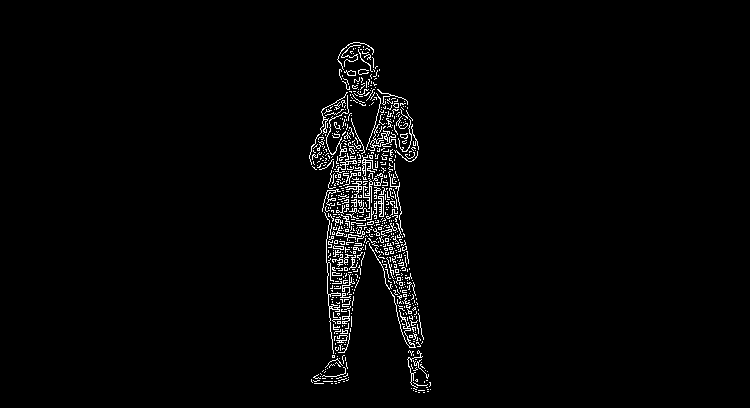
\includegraphics[scale=0.4]{anhtimcanh.png}}
\caption{Ảnh với các cạnh đã tìm được.}
\label{fig}
\end{figure}
 \FloatBarrier
\subsection{Tìm đường viền lớn nhất}
Đây là bước quan trọng nhất, quyết định chất lượng của ảnh sau khi xóa nền, thuật toán tìm đường viền bằng cách nối các cạnh liền nhau bao quanh đối tượng và tìm ra đường viền lớn nhất và xem đối tượng trong đường viền lớn nhất đó là chủ thể ta cần giữ lại.
\begin{figure}[!htb]
\centerline{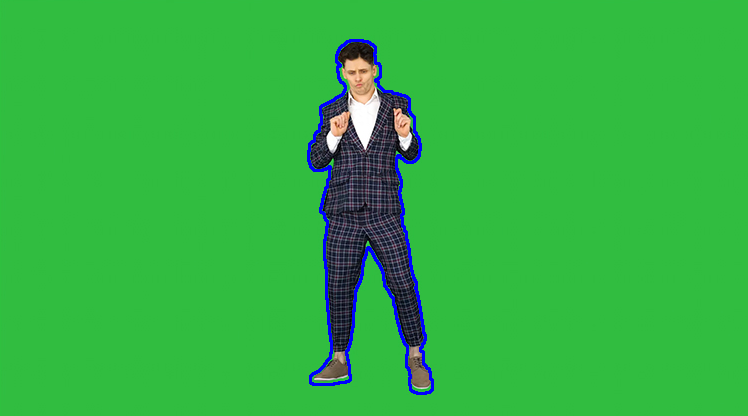
\includegraphics[scale=0.4]{anhdvln.png}}
\caption{Ảnh với đường viền lớn nhất đã tìm được.}
\label{fig}
\end{figure}
 \FloatBarrier
\subsection{Xóa phần bên ngoài đường viền lớn nhất}
Tiến hành xóa phần hình bên ngoài đường viền lớn nhất vừa tìm được và giữ lại đối tượng ta coi là chủ thể bên trong đường viền lớn nhất đó. Kết quả ta được ảnh đã xóa nền.
\begin{figure}[!htb]
\centerline{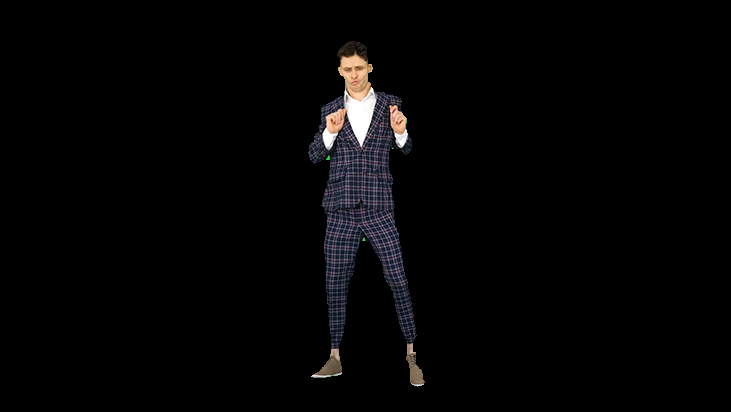
\includegraphics[scale=0.4]{anhkq.png}}
\caption{Kết quả sau khi xóa phần hình bên ngoài đường viền lớn nhất.}
\label{fig}
\end{figure}
 \FloatBarrier
 \section{Ưu, nhược điểm và hướng phát triển}
 \subsection{Ưu điểm}
 \begin{enumerate}
     \item Ý tưởng đơn giản, dễ hiểu.
     \item Dễ thực hiện.
     \item Cho kết quả khá tốt trên những bức ảnh có chủ thể tách biệt với nền (như ảnh chromakey)/
 \end{enumerate}
 \subsection{Nhược điểm và hướng phát triển}
 \begin{enumerate}
     \item Phương pháp này cho hiệu quả rất tệ trên các bức ảnh có nền nhiều cạnh hoặc nền có màu tương đồng với chủ thể, hoặc ảnh có độ tương phản thấp: trường hợp nền có nhiều cạnh hoặc nền có màu tương đồng với chủ thể, hoặc ảnh đầu vào có độ tương phản thấp làm cho thuật toán tìm đường viền lớn nhất ghép luôn các cạnh tìm được ở nền vào đường viền lớn nhất, do đó ảnh sau khi xóa nền vẫn chứa một phần nền.
\begin{figure}[!htb]
\centerline{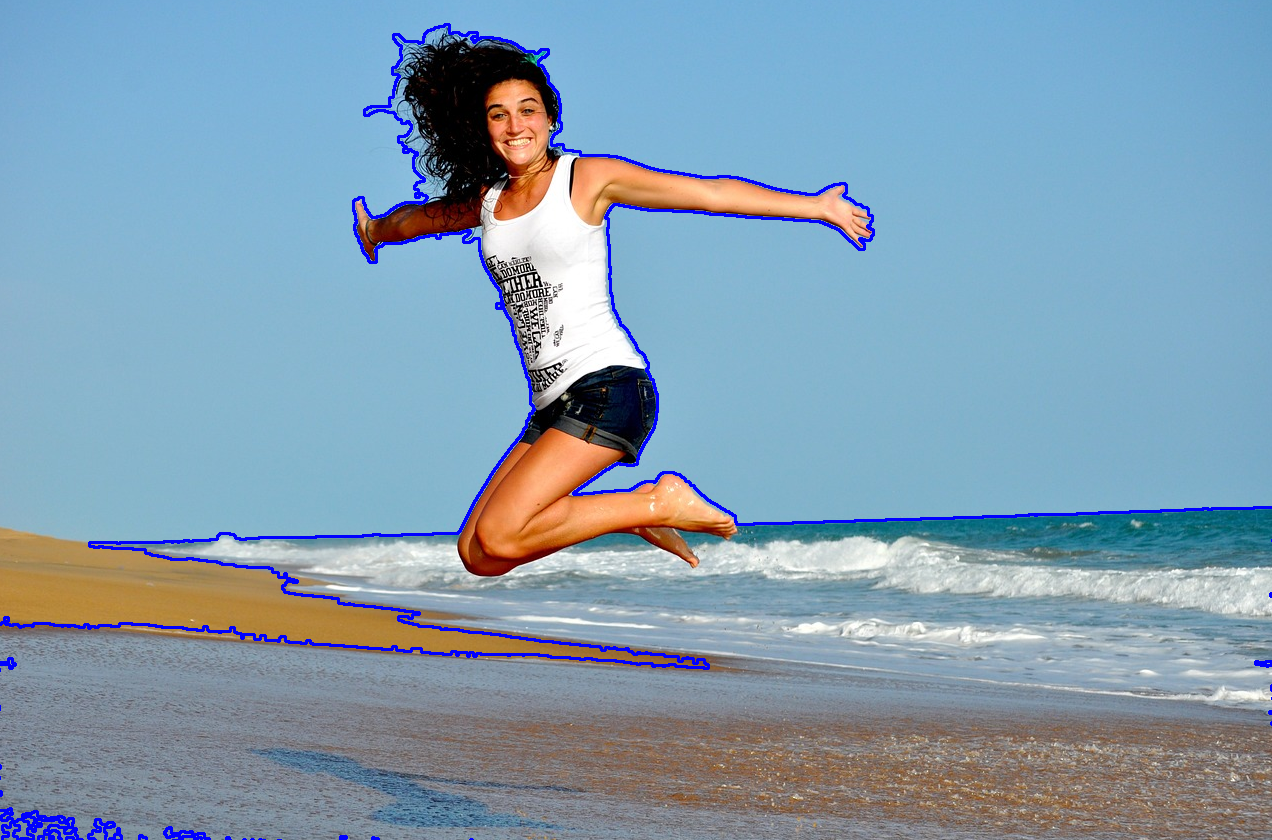
\includegraphics[scale=0.22]{anhnd1.png}}
\caption{Đường viền lớn nhất tìm được trên ảnh có nền phức tạp.}
\label{fig}
\end{figure}
 \FloatBarrier
 \begin{figure}[!htb]
\centerline{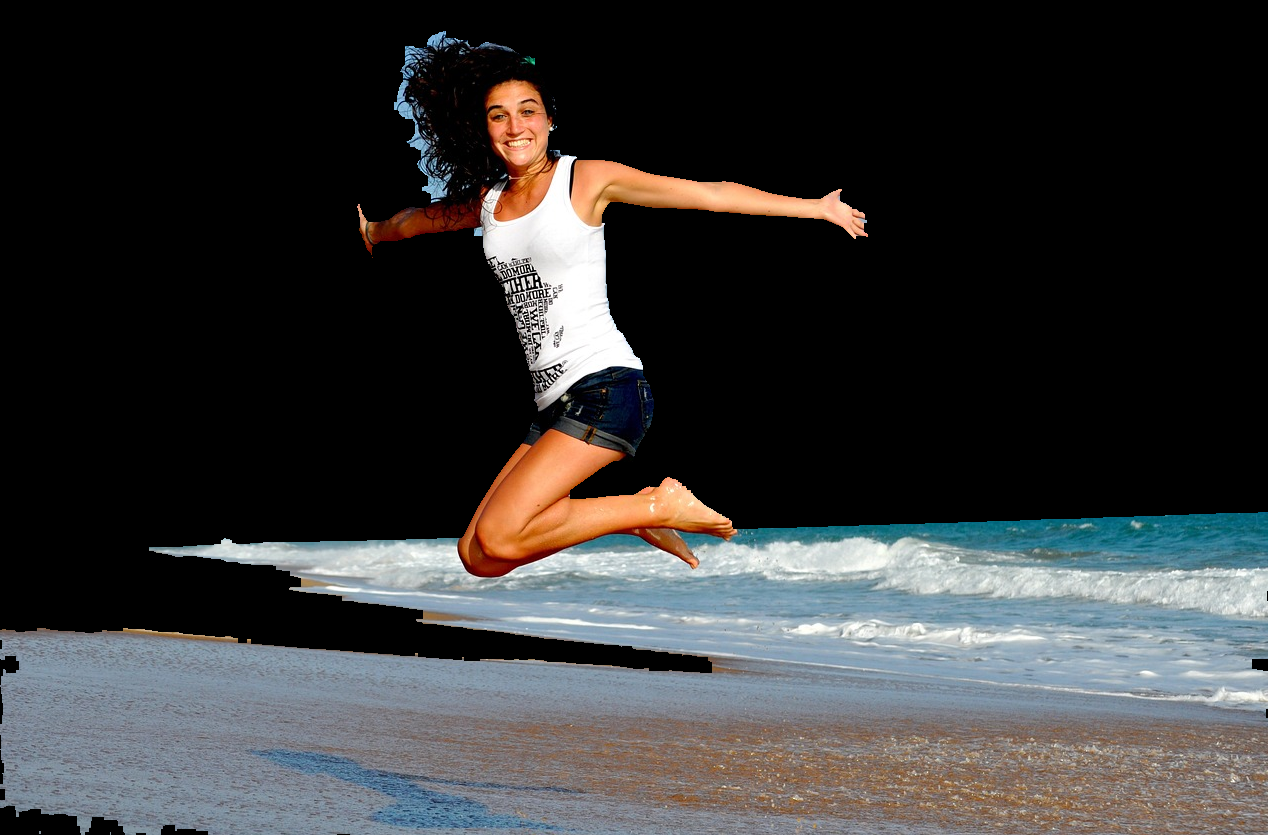
\includegraphics[scale=0.22]{anhnd2.png}}
\caption{Kết quả sau khi xóa nền ảnh có nền phức tạp.}
\label{fig}
\end{figure}
 \FloatBarrier
  Đây là nhược điểm chung của các phương pháp xóa nền sử dụng các phương pháp xử lý ảnh cơ bản nên không có cách khắc phục triệt để cho nhược điểm này, để khắc phục một cách triệt để thì ta vẫn phải sử dụng Máy học.
\item Trường hợp nền xuất hiện trong chủ thể đồng nghĩa với việc nền nằm trong đường viền lớn nhất bao quanh chủ thể mà ta tìm được, nên phần nền ấy sẽ không được xóa.
 \begin{figure}[!htb]
\centerline{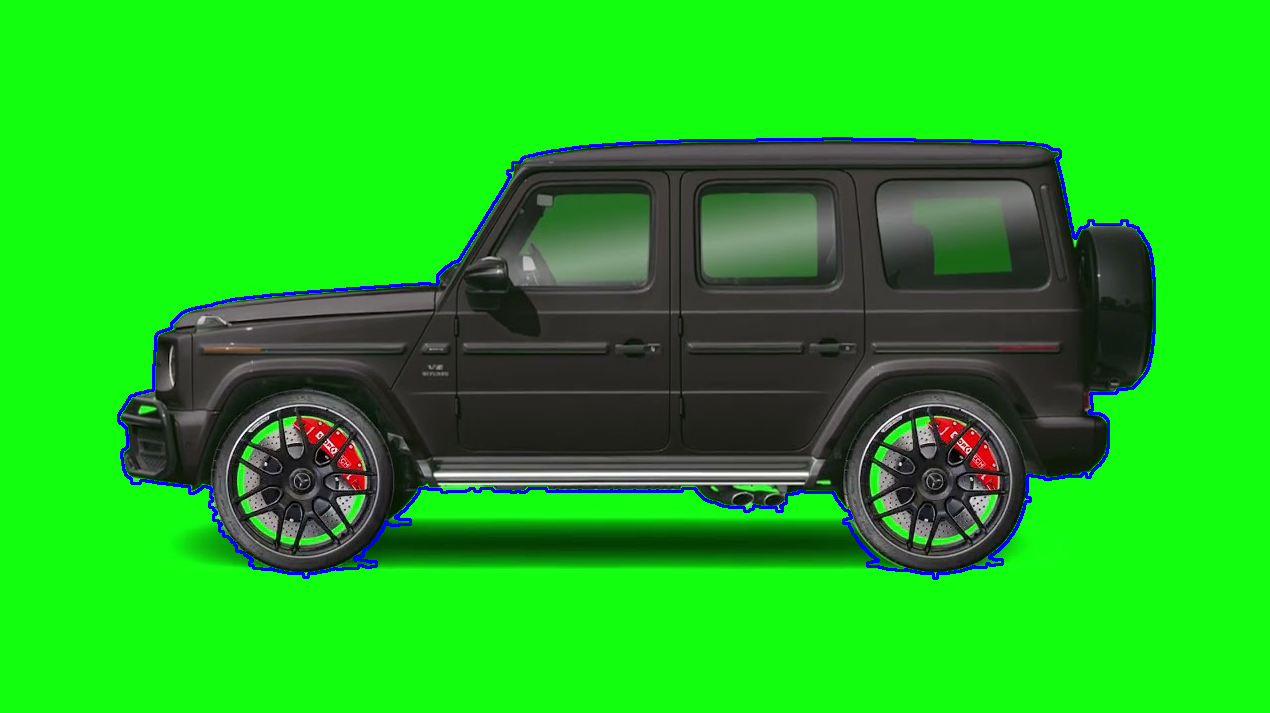
\includegraphics[scale=0.22]{anhnd3.png}}
\caption{Đường viền lớn nhất tìm được trên ảnh có nền trong chủ thể.}
\label{fig}
\end{figure}
 \FloatBarrier
 \begin{figure}[!htb]
\centerline{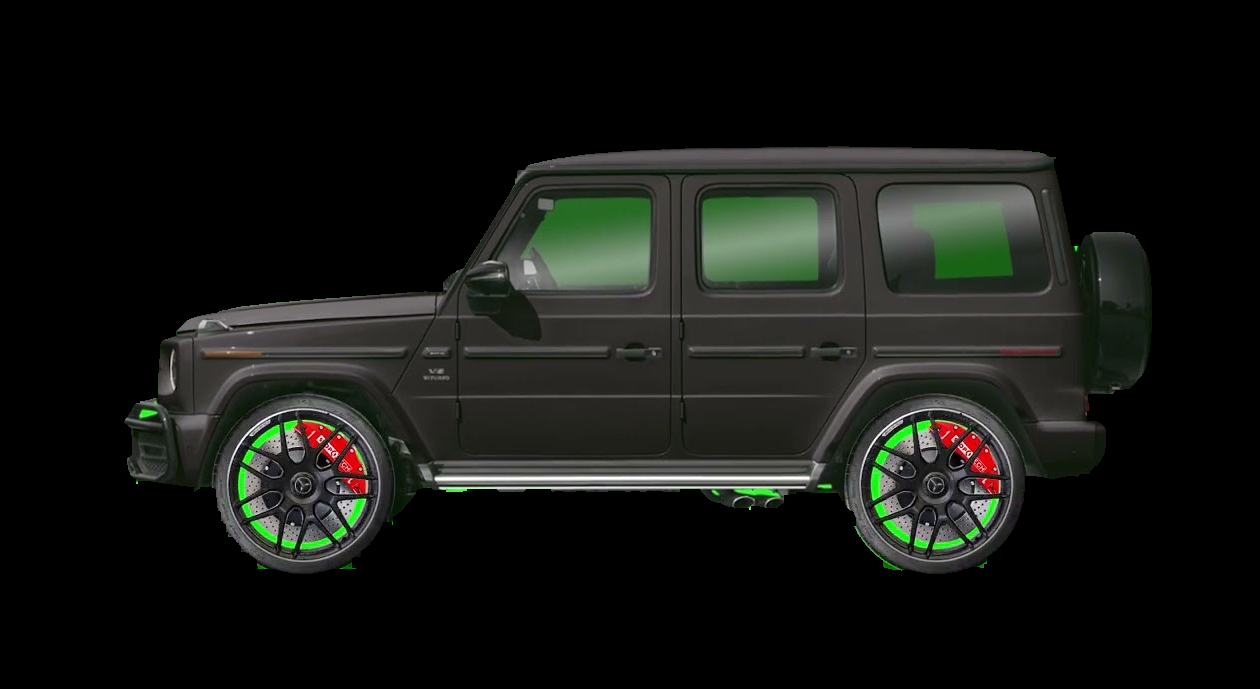
\includegraphics[scale=0.22]{anhnd4.png}}
\caption{Kết quả sau khi xóa nền ảnh có nền trong chủ thể.}
\label{fig}
\end{figure}
 \FloatBarrier
Ta có thể giải quyết nhược điểm này bằng một thuật toán cao cấp hơn: thuật toán phân đoạn Watershed (thuật toán phân đoạn Watershed xem ảnh xám như một cấu trúc địa hình với các pixel cường độ cao
biểu thị đỉnh đồi trong khi các pixel cường độ thấp biểu thị thung lũng, sau đó thuật toán tiến hành làm ngập các thung lũng, Khi nước dâng lên, tùy thuộc vào các đỉnh, nước từ các thung lũng khác nhau sẽ bị hợp nhất, để ngăn điều này, thuật toán xây dựng các “rào cản” ở những nơi nước bị hợp nhất. Tiếp tục đổ đầy nước và xây dựng các “rào cản” cho đến khi nước ngập khắp các đỉnh. Kết thúc thuật toán, các “rào cản” ta đã xây dựng chính là kết quả phân đoạn).
\item Có thể không phát hiện được đường viền do các cạnh tìm được không tạo thành đường cong khép kín.
\item Trường hợp ảnh có nhiều đối tượng rời rạc (không nằm chồng lên nhau), phương pháp này chỉ có thể phát hiện được một đối tượng.
 \end{enumerate}
 Ta có thể giải quyết cả 2 nhược điểm (3), (4) cũng như cải thiện chất lượng ảnh xóa nền của thuật toán bằng phép Dilate và Erode.
  \begin{figure}[!htb]
\centerline{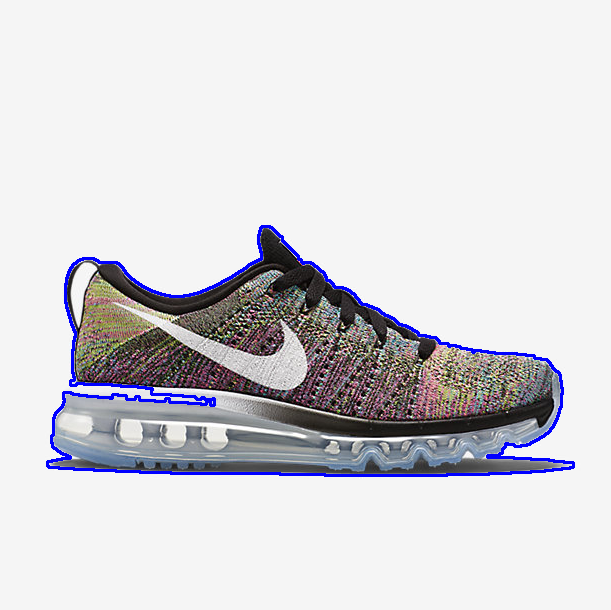
\includegraphics[scale=0.5]{anhnd5.png}}
\caption{Đường viền lớn nhất tìm được trên ảnh chiếc giày.}
\label{fig}
\end{figure}
 \FloatBarrier
   \begin{figure}[!htb]
\centerline{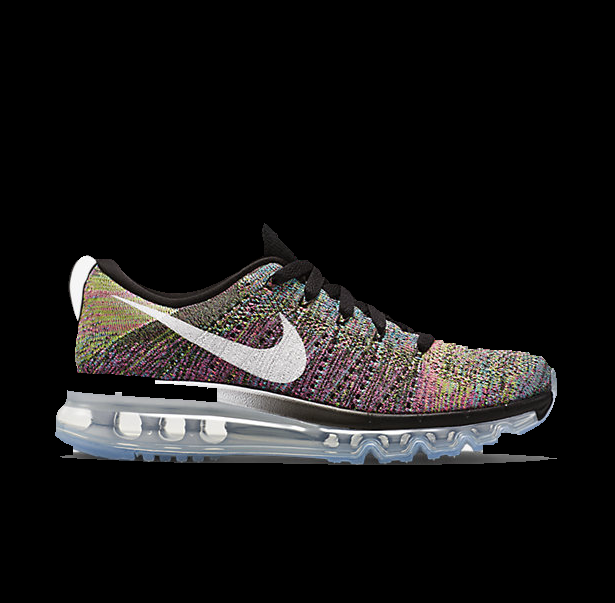
\includegraphics[scale=0.5]{anhnd6.png}}
\caption{Kết quả xóa nền ảnh chiếc giày.}
\label{fig}
\end{figure}
 \FloatBarrier
Ta nhận thấy được ở hình 10 và 11, phần gần đế giày do có màu trắng trùng màu với phần nền nên các thuật toán tìm cạnh không tìm được cạnh ở đó nên đường viền lớn nhất tìm được không bao gồm cạnh đó. Ta sử dụng phép biến đổi Dilate để làm đầy cạnh đó, giúp cho thuật toán tìm đường viền tìm ra được đầy đủ đường viền bao quanh chiếc giày, sau đó lại dùng phép Erode để làm mượt phần đường viền để cho ra kết quả đẹp hơn.

 \begin{figure}[!htb]
\centerline{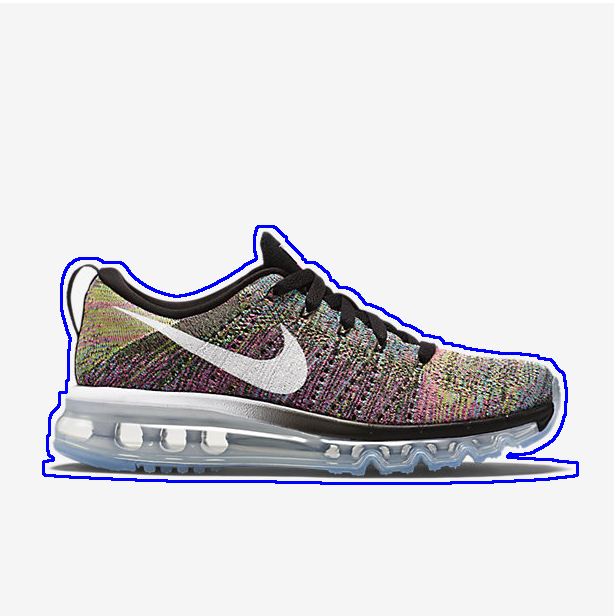
\includegraphics[scale=0.5]{anhnd7.png}}
\caption{Đường viền lớn nhất tìm được trên ảnh chiếc giày sau phép Dilate.}
\label{fig}
\end{figure}
 \FloatBarrier
   \begin{figure}[!htb]
\centerline{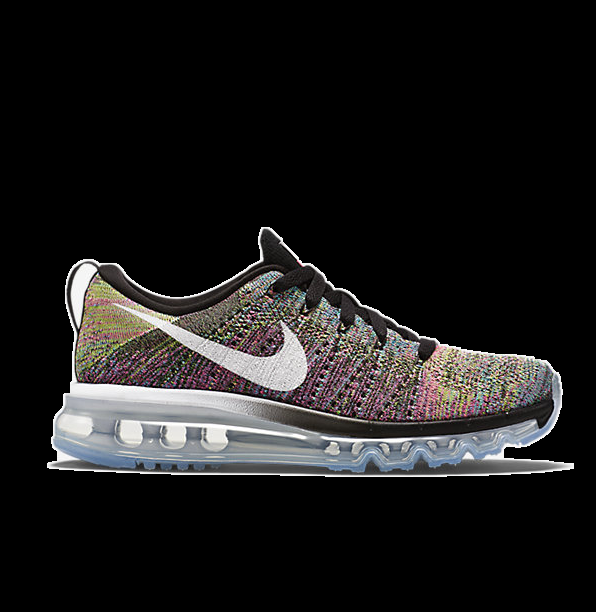
\includegraphics[scale=0.5]{anhnd8.png}}
\caption{Kết quả xóa nền ảnh chiếc giày sử dụng phép Dilate và Erode.}
\label{fig}
\end{figure}
 \FloatBarrier
 Đến với ví dụ tiếp theo khi ảnh có nhiều đối tượng rời rạc (không nằm chồng lên nhau).
 \begin{figure}[!htb]
\centerline{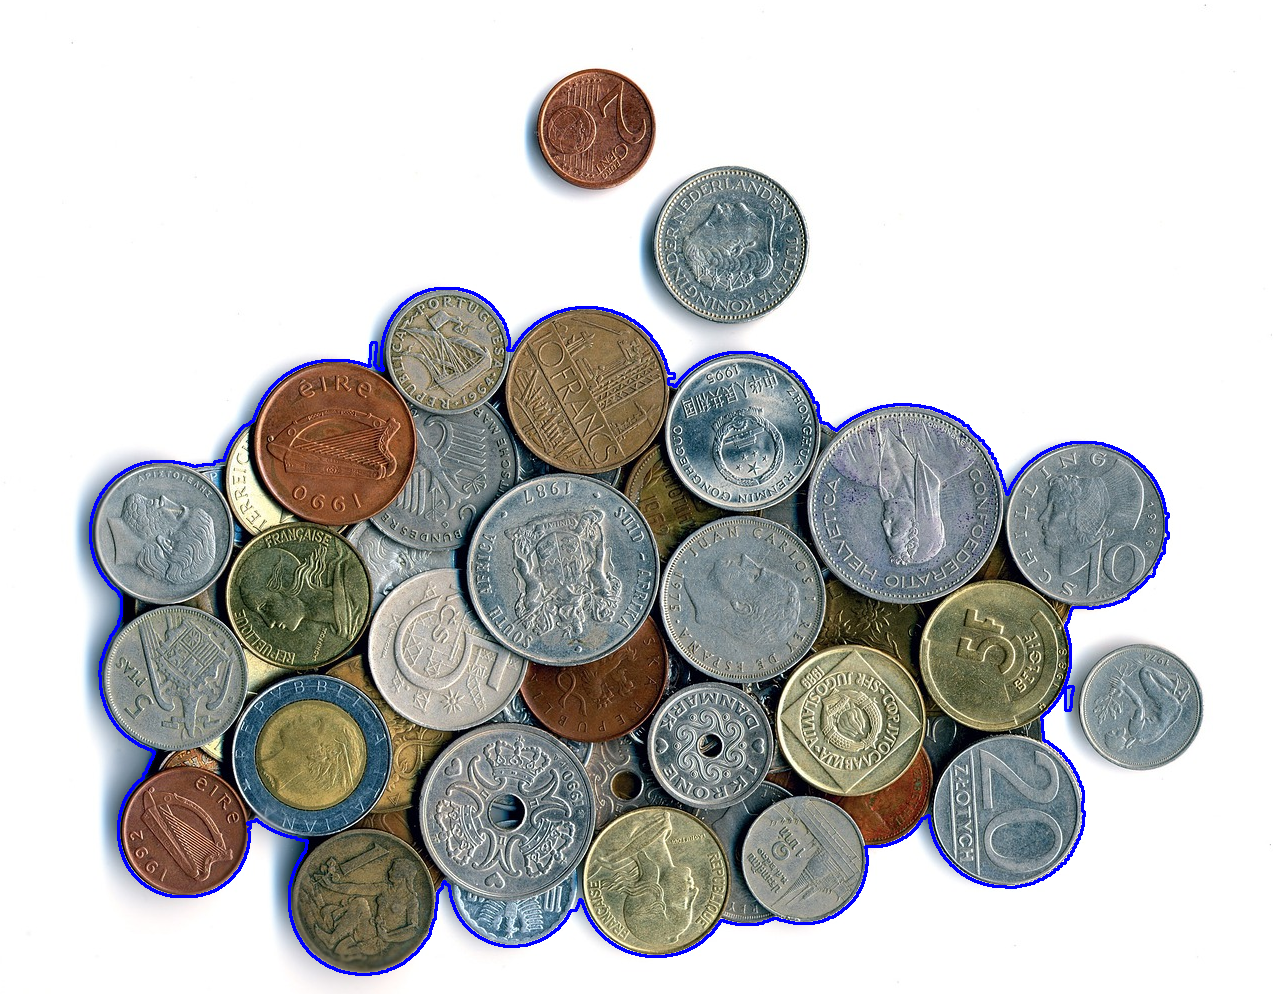
\includegraphics[scale=0.22]{anhnd9.png}}
\caption{Đường viền lớn nhất tìm được trên ảnh đồng xu.}
\label{fig}
\end{figure}
 \FloatBarrier
  \begin{figure}[!htb]
\centerline{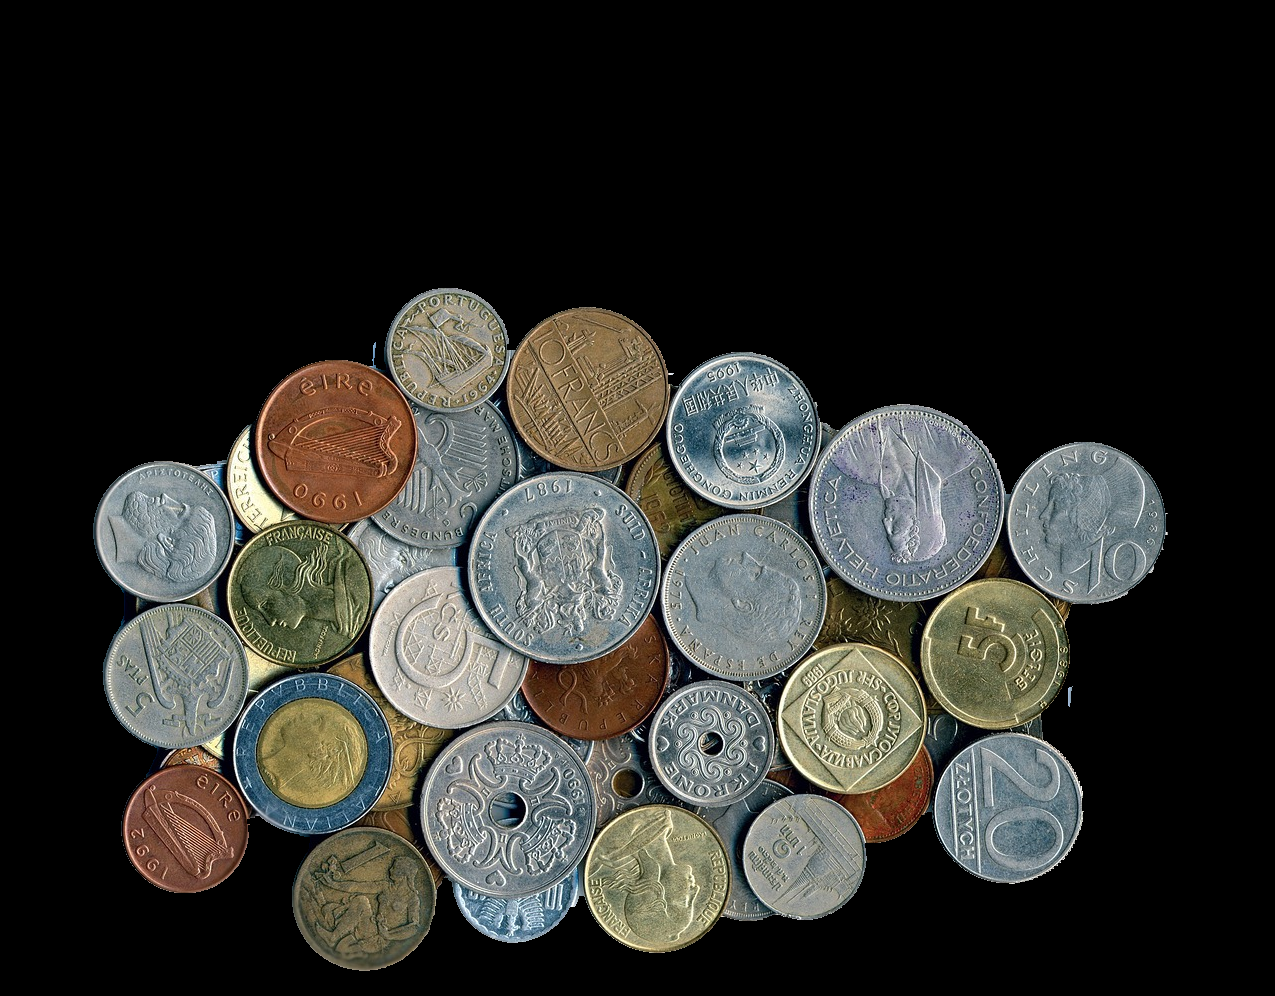
\includegraphics[scale=0.22]{anhnd10.png}}
\caption{Kết quả xóa nền trên ảnh đồng xu.}
\label{fig}
\end{figure}
 \FloatBarrier
 Ta sử dụng phép Dilate để làm đầy cạnh sao cho đường viền bao trùm cả hai đồng xu phía trên, sau đó dùng phép Erode để xói mòn những phần thừa mà phép Dilate để lại.
 \begin{figure}[!htb]
\centerline{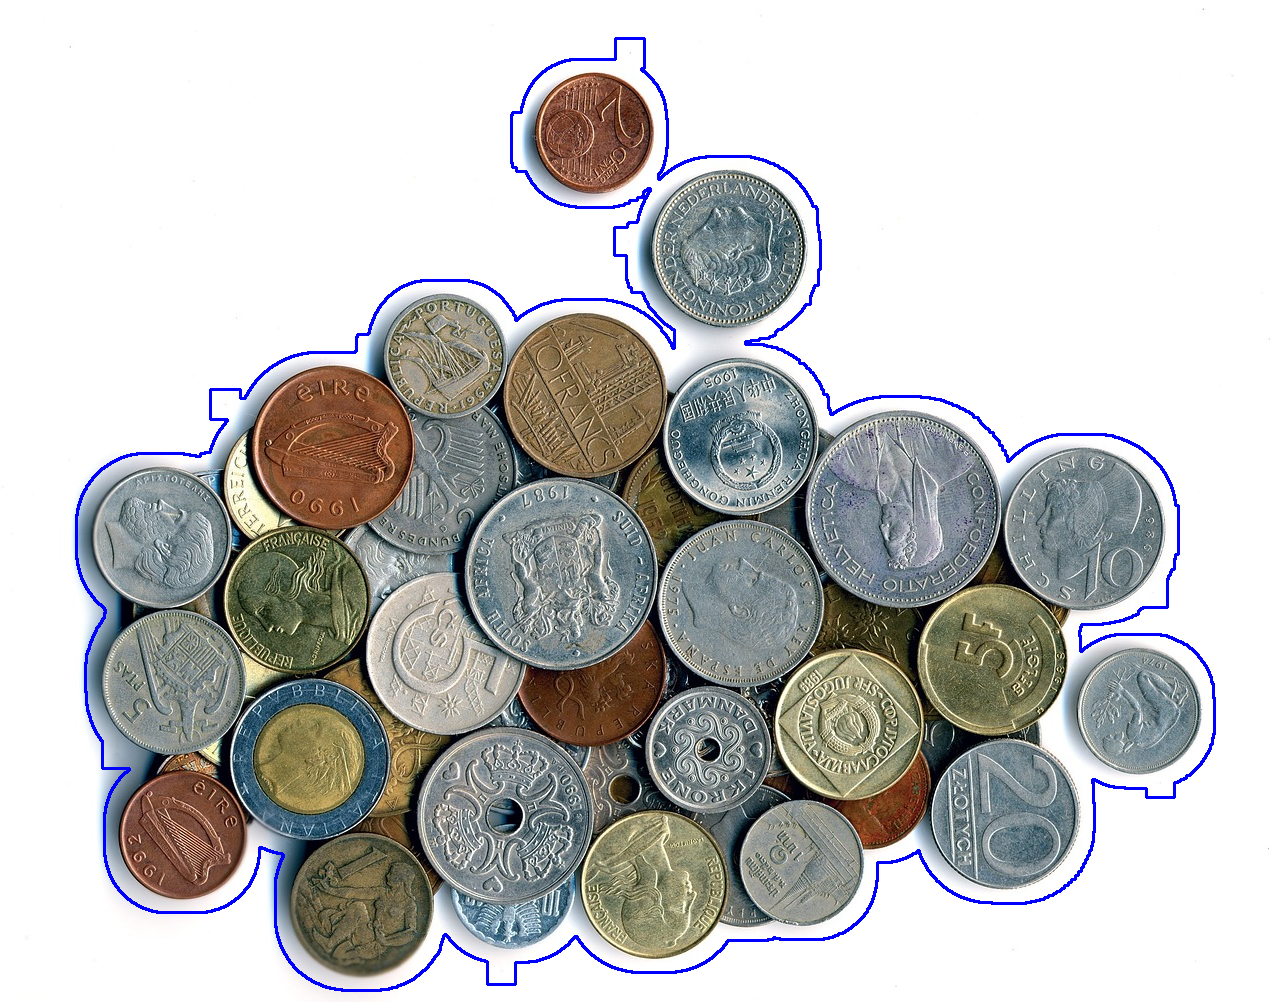
\includegraphics[scale=0.22]{anhnd11.png}}
\caption{Đường viền lớn nhất tìm được trên ảnh đồng xu sau phép Dilate.}
\label{fig}
\end{figure}
 \FloatBarrier
  \begin{figure}[!htb]
\centerline{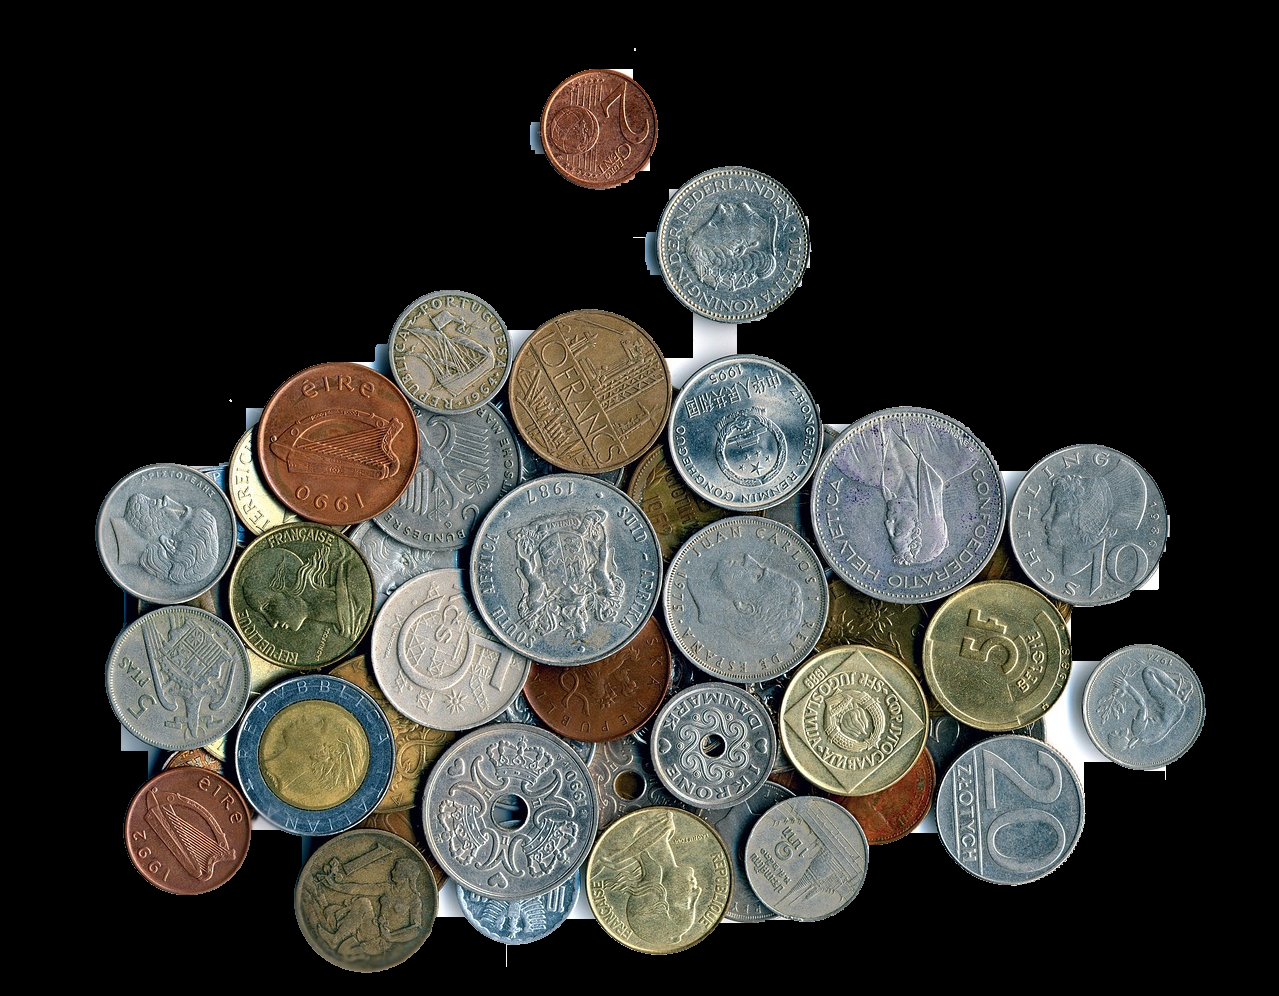
\includegraphics[scale=0.22]{anhnd12.png}}
\caption{Kết quả xóa nền trên ảnh đồng xu sử dụng phép Dilate và Erode.}
\label{fig}
\end{figure}
 \FloatBarrier
 Qua hai ví dụ trên ta thấy được hai phép Dilate và Erode cải thiện đáng kể chất lượng của ảnh xóa nền cũng như giải quyết được nhược điểm cố hữu của phương pháp.
\section{So sánh với các phương pháp khác}
  \begin{figure}[!htb]
\centerline{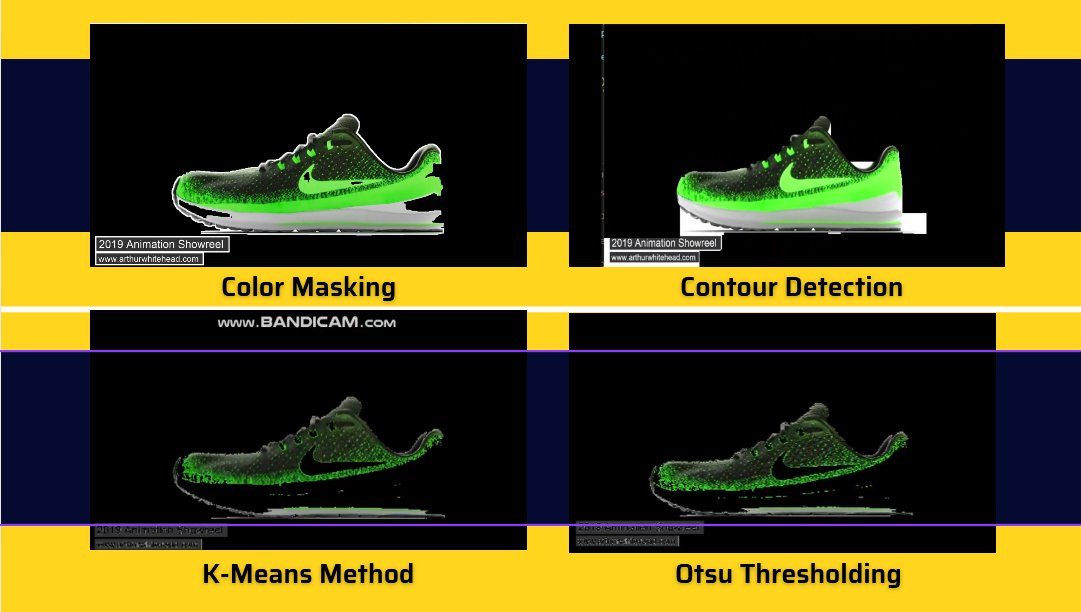
\includegraphics[scale=0.3]{anhss1.png}}
\caption{Kết quả của các phương pháp trên ảnh đơn giản.}
\label{fig}
\end{figure}
 \FloatBarrier
 Ở ảnh đơn giản, Contour Detection cho kết quả khá tốt so với K-Means Method và Otsu Thresholding. Tuy nhiên lại lép vế một chút so với Color Masking.
  \begin{figure}[!htb]
\centerline{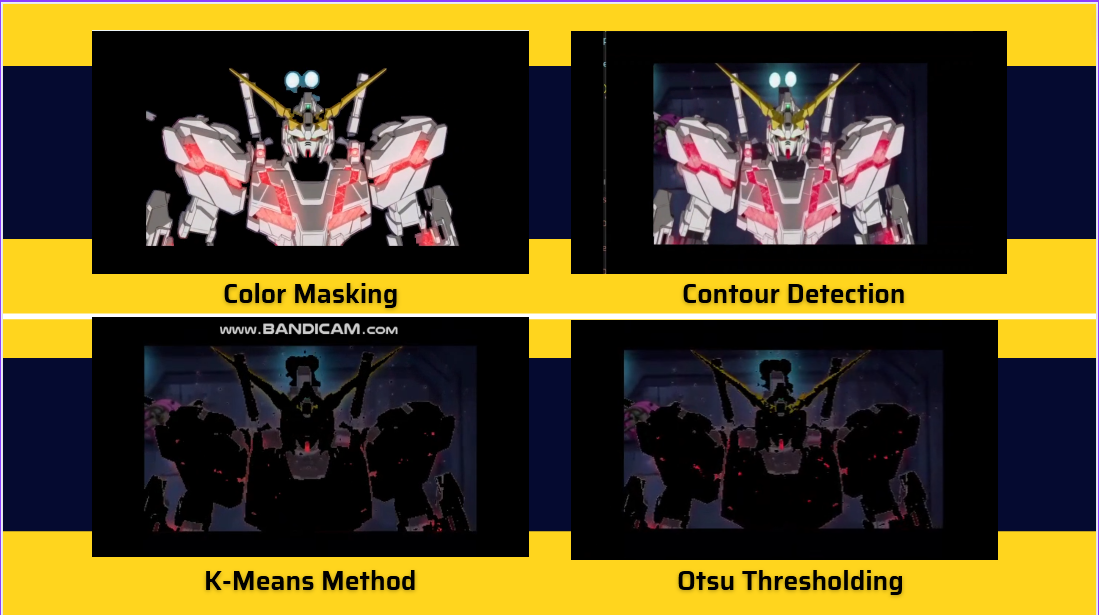
\includegraphics[scale=0.3]{anhss2.png}}
\caption{Kết quả của các phương pháp trên ảnh phức tạp.}
\label{fig}
\end{figure}
 \FloatBarrier
 Đối với ảnh phức tạp, Color Masking vẫn cho ra kết quả khá tốt, do ảnh có một đường viền bao quanh khung hình nên Contout Detection nghĩ đây là đường viền chứa đối tượng và lấy luôn đường viền này nên kết quả cho ra không khác so với ảnh gốc. K-Means Method và Otsu Thresholding cho kết quả không được tốt lắm trên các ảnh phức tạp.
 \FloatBarrier
 \begin{table}[htbp]
 \caption{Bảng so sánh FPS của các phương pháp}
\begin{center}
\begin{tabular}{|l|cccc|}
\hline
             & \multicolumn{4}{c|}{\textbf{Phương pháp}}                                                                                                                                                                                                                                                                      \\ \hline
             & \multicolumn{1}{c|}{\begin{tabular}[c]{@{}c@{}}Color\\  Masking\end{tabular}} & \multicolumn{1}{c|}{\begin{tabular}[c]{@{}c@{}}Contour\\ Detection\end{tabular}} & \multicolumn{1}{c|}{\begin{tabular}[c]{@{}c@{}}K-Means\\ Method\end{tabular}} & \begin{tabular}[c]{@{}c@{}}Otsu\\ Thresholding\end{tabular} \\ \hline
\textbf{FPS} & \multicolumn{1}{c|}{21}                                                       & \multicolumn{1}{c|}{16}                                                          & \multicolumn{1}{c|}{12}                                                       & 24                                                          \\ \hline
\end{tabular}
\end{center}
\end{table}
Ngoài ra dựa vào bảng khung hình trên giây (FPS), ta thấy được thuật toán Otsu Threholding cho hiệu suất xử lý cao nhất, tiếp đến là Color Masking, đứng thứ ba là Contour Detection và tệ nhất là K-Means Method.
Ưu điểm của cả 4 phương pháp này là dễ cài đặt và sử dụng, phương pháp đơn giản và dễ hiểu. Tuy nhiên cũng như các phương pháp xóa nền không dùng Máy học khác, cả 4 phương pháp này đều chỉ cho ra kết quả tốt nhất trên các ảnh không quá phức tạp.
\section{Tổng kết}
 Xóa nền sử dụng Contour Detection là phương pháp xóa nền đơn giản, dễ hiểu, không sử dụng đến Máy học, cho hiệu quả cao trên những ảnh có chủ thể tách biệt với nền (như các ảnh nền xanh). Tuy nhiên phương pháp này lại bộc lộ rõ những khuyết điểm của mình trên những bức ảnh thực tế khi ảnh có nền phức tạp. Nhìn chung, phương pháp này thích hợp cho các ảnh đã được xử lý hậu trường chứ không thích hợp với những bức ảnh ngoài thực tế. 
\begin{thebibliography}{00}
\bibitem{b1} \url{https://en.wikipedia.org/wiki/Foreground_detection}}
\bibitem{b2} \url{https://machinelearningknowledge.ai/image-segmentation-in-python-opencv/#ii_Contour_Detection}
\bibitem{b3} \url{https://bleedai.com/contour-detection-101-the-basics-pt1/}
\bibitem{b4} \url{https://learnopencv.com/contour-detection-using-opencv-python-c/}
\bibitem{b5} \url{https://docs.opencv.org/4.x/d3/db4/tutorial_py_watershed.html}
\bibitem{b6} \url{https://docs.opencv.org/3.4/d4/d73/tutorial_py_contours_begin.html}
\bibitem{b7} \url{https://www.banuba.com/blog/background-subtraction-guide}
\end{thebibliography}

\end{document}
